\documentclass{article}

\usepackage{pandekten}
\usepackage{dashrule}

\makeatletter
\newcommand*{\shifttext}[1]{%
  \settowidth{\@tempdima}{#1}%
  \hspace{-\@tempdima}#1%
}
\newcommand{\plabel}[1]{%
\shifttext{\textbf{#1}\quad}%
}
\newcommand{\prule}{%
\begin{center}%
\hdashrule[0.5ex]{.99\linewidth}{1pt}{1pt 2.5pt}%
\end{center}%
}

\makeatother

\newcommand{\minusbaseline}{\abovedisplayskip=0pt\abovedisplayshortskip=0pt~\vspace*{-\baselineskip}}%

\setlength{\parindent}{0pt}

\title{Assignment 10}
\author{Ze Chen}

\begin{document}

\maketitle

\plabel{1 (a)}%
Global symmetries are $\phi\rightarrow e^{i\alpha}\phi$, $\phi \rightarrow \overline{\phi}$, spacetime translation and rotation.
The space of vacua are parametrized by $\phi_0 = v e^{i\theta}$.
Writing
\[ \phi = v + \frac{1}{\sqrt{2}}(\sigma(x) + i\pi(x)) \]
we find
\begin{align*}
    \mathcal{L} &= \frac{1}{2}(\partial \sigma)^2 + \frac{1}{2}(\partial \pi)^2 - \frac{1}{2} \lambda v^2 \sigma^2 \\
    &\phantom{{}={}} - \frac{\lambda v}{2\sqrt{2}}\sigma^3 - \frac{\lambda v}{2\sqrt{2}} \sigma\pi^2 - \frac{\lambda}{16}\sigma^4 - \frac{\lambda}{8} \sigma^2 \pi^2 - \frac{\lambda}{16}\pi^4.
\end{align*}
The $\sigma$ particle has mass $m_\sigma^2 = \lambda v^2$ while $\pi$ is massless.
The Feynman diagrams are given below.
\begin{itemize}
    \item Vertices:
    \begin{center}
        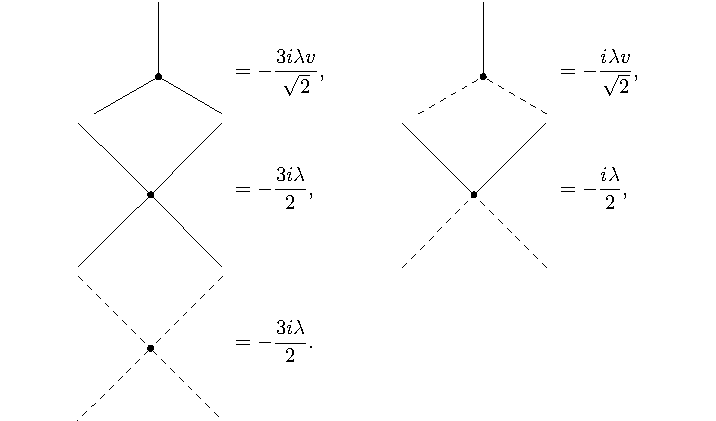
\includegraphics{img/cartesian/vertex/vertex.pdf}
    \end{center}
    \item Propagators:
    \begin{center}
        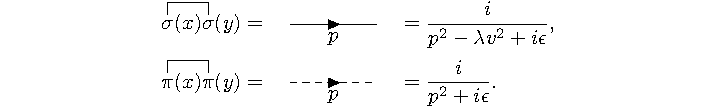
\includegraphics{img/cartesian/propagator/propagator.pdf}
    \end{center}
\end{itemize}
The decay $\sigma \rightarrow \pi + \pi$ has $\abs{\mathcal{M}}^2 = \lambda^2 v^2/2$.
Therefore, since $\abs{\vb{p}} = m_\sigma/2$,
\[ \Gamma = \frac{\abs{\vb{p}}}{16 \pi m_\sigma^2} \abs{\mathcal{M}}^2 = \frac{\lambda^2 v^2}{64\pi m_\sigma}. \]
The tree-level diagram of $\pi+\pi\rightarrow \pi+\pi$ is given below.
\begin{center}
    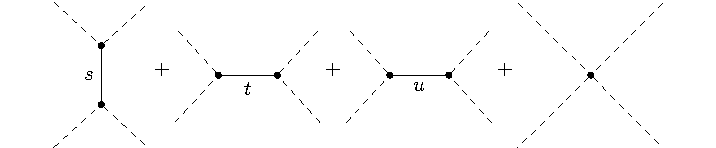
\includegraphics{img/cartesian/scatter/scalar.pdf}
\end{center}
The amplitude is given by
\[ i\mathcal{M} = -\frac{i\lambda^2 v^2}{2}\qty(\frac{1}{s - m_\sigma^2} + \frac{1}{t - m_\sigma^2} + \frac{1}{u - m_\sigma^2}) - \frac{3i\lambda}{2}. \]

\plabel{(b)}%
Writing
\[ \phi = \rho e^{i\theta}, \quad \rho = v + \frac{h}{\sqrt{2}}, \]
we find
\begin{align*}
    \mathcal{L} &= \frac{1}{2}(\partial h)^2 + \frac{1}{2}(\sqrt{2}v \partial \theta)^2 - \frac{1}{2}\lambda v^2 h^2 \\
    &\phantom{{}={}} - \frac{\lambda v}{2\sqrt{2}} h^3 + \frac{1}{\sqrt{2}v} h (\sqrt{2}v \partial \theta)^2 - \frac{\lambda}{16} h^4 + \frac{1}{4v^2} h^2 (\sqrt{2}v\partial \theta)^2.
\end{align*}
The $h$ particle has mass $m_h^2 = \lambda v^2$ while $\theta$ is massless.
The Feynman rules are given below.
\begin{itemize}
    \item Propagators:
    \begin{center}
        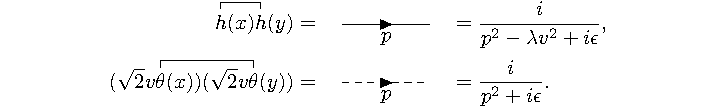
\includegraphics{img/polar/propagator/propagator.pdf}
    \end{center}
    \item Vertices:
    \begin{center}
        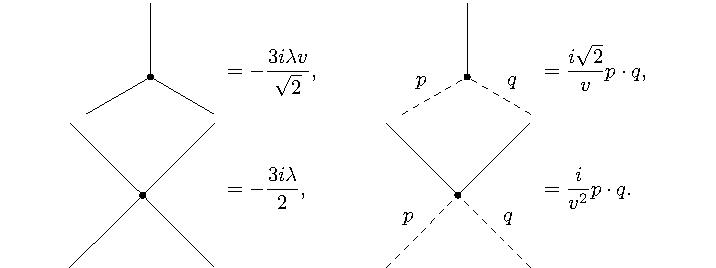
\includegraphics{img/polar/vertex/vertex.pdf}
    \end{center}
\end{itemize}
The decay $\sigma\rightarrow\theta + \theta$ has
\[ \abs{\mathcal{M}}^2 = \qty(\frac{\sqrt{2}}{v} p\cdot q)^2 = \frac{2}{v^2}\qty(\frac{m_h^2}{2})^2 = \frac{\lambda^2 v^2}{2}. \]
Therefore,
\[ \Gamma = \frac{\abs{\vb{p}}}{16 \pi m_\sigma^2} \abs{\mathcal{M}}^2 = \frac{\lambda^2 v^2}{64\pi m_\sigma}. \]

\plabel{(c)}%
The Lagrangian is given by
\[ \mathcal{L} = -\frac{1}{4} F_{\mu\nu}F^{\mu\nu} + (D_\mu\phi)^*(D_\mu\phi) - \frac{\lambda}{4}(\phi^* \phi - v^2)^2, \]
where
\[ D_\mu = \partial_\mu + ieA_\mu. \]
The symmetries are those described in (a), plus the gauge symmetry
\[ \phi(x) \rightarrow e^{i\alpha(x)}\phi(x),\quad A_\mu(x) \rightarrow A_\mu(x) - \frac{1}{e} \partial_\mu \alpha(x). \]
Writing
\[ \phi = \rho e^{i\theta}, \quad \rho = v + \frac{h}{\sqrt{2}}, \]
we find
\begin{align*}
    \mathcal{L} &= -\frac{1}{4} F_{\mu\nu}F^{\mu\nu} + \frac{1}{2}(\partial h)^2  - \frac{1}{2}\lambda v^2 h^2 - \frac{\lambda v}{2\sqrt{2}} h^3 - \frac{\lambda}{16} h^4  \\
    &\phantom{{}={}} + \frac{1}{2}(h+\sqrt{2}v)^2 (eA + \partial\theta)^2.
\end{align*}
The $\partial \theta$ may be elimiated by a gauge transformation, leaving
\begin{align*}
    \mathcal{L} &= -\frac{1}{4} F_{\mu\nu}F^{\mu\nu} + \frac{1}{2} (2 v^2e^2) A_\mu A^\mu + \frac{1}{2}(\partial h)^2  - \frac{1}{2}\lambda v^2 h^2   \\
    &\phantom{{}={}} - \frac{\lambda v}{2\sqrt{2}} h^3 + \sqrt{2}ve^2 A_\mu A^\mu h - \frac{\lambda}{16} h^4 + \frac{1}{2}e^2 A_\mu A^\mu h^2.
\end{align*}
The $h$ particle has mass $m^2_h = \lambda v^2$ while $A_\mu$ has mass $m_A^2 = 2v^2 e^2$.
The massless particle $\theta$ is eliminated and $A_\mu$ acquires a mass.

\plabel{(d)}%
The Feynman rules are given below.
\begin{itemize}
    \item Propagators:
    \begin{center}
        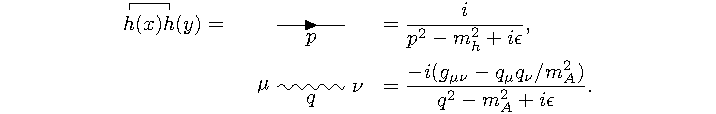
\includegraphics{img/u1/propagator/propagator.pdf}
    \end{center}
    \item Vertices:
    \begin{center}
        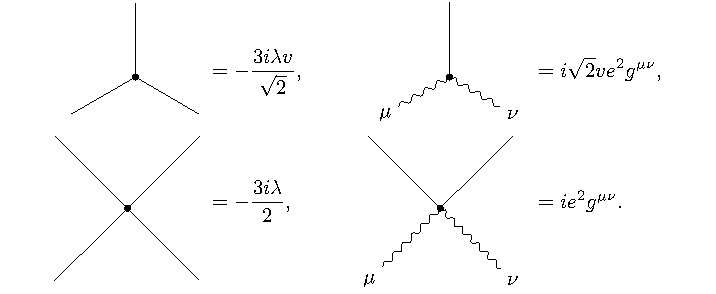
\includegraphics{img/u1/vertex/vertex.pdf}
    \end{center}
\end{itemize}
The amplitude and decay rate of $h\rightarrow A+A$ are given by
\begin{align*}
    \abs{\mathcal{M}}^2 &= \sum_{\epsilon^{(1)},\epsilon^{(2)}} \abs{\epsilon^{(1)*}_\mu (\sqrt{2}ve^2 g^{\mu\nu}) \epsilon^{(2)*}_\nu}^2 \\
    &= 2v^2 e^4 \qty(2+\qty(\frac{q^{(1)}\cdot q^{(2)}}{m_A^2})^2) \\
    &= 2v^2 e^4\qty(2+\qty(\frac{m_h^2/2 - m_A^2}{m_A^2})^2), \\
    \Gamma &= \frac{\sqrt{m_h^2 - 4m_A^2}}{32\pi m_h^2}\abs{\mathcal{M}}^2 = \frac{\sqrt{m_h^2 - 4m_A^2}}{16\pi m_h^2}v^2 e^4\qty(2+\qty(\frac{m_h^2/2 - m_A^2}{m_A^2})^2).
\end{align*}
The decay is allowed if $m_h>2m_A$.
\par
The tree-level diagrams for the process $A+A\rightarrow A+A$ are given below.
\begin{center}
    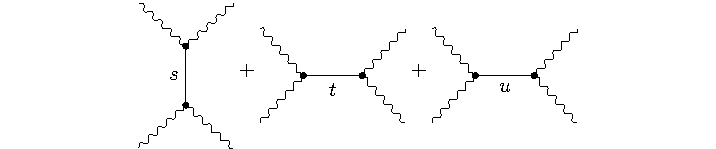
\includegraphics{img/u1/scatter/scalar.pdf}
\end{center}
The amplitude is given by
\[ \mathcal{M} = -2i v^2 e^4 \epsilon_\rho^{(3)*}\epsilon_\sigma^{(4)*}\qty(\frac{g^{\mu\nu}g^{\rho\sigma}}{s - m_h^2} + \frac{g^{\mu\rho}g^{\nu\sigma}}{t - m_h^2} + \frac{g^{\mu\sigma}g^{\nu\rho}}{u - m_h^2})\epsilon_\mu^{(1)}\epsilon_\nu^{(2)}. \]
There is no $A^4$ vertex.

\plabel{(e)}%
We add a Yukawa interaction and electromagnetic interaction.
\begin{align*}
    \mathcal{L} &= -\frac{1}{4} F_{\mu\nu}F^{\mu\nu} + \frac{1}{2} (2 v^2e^2) A_\mu A^\mu + \frac{1}{2}(\partial h)^2  - \frac{1}{2}\lambda v^2 h^2 + \overline{\psi}(i\slashed{\partial}-m_\psi)\psi \\
    &\phantom{{}={}} - \frac{\lambda v}{2\sqrt{2}} h^3 + \sqrt{2}ve^2 A_\mu A^\mu h - \frac{\lambda}{16} h^4 + \frac{1}{2}e^2 A_\mu A^\mu h^2 - g_1 \overline{\psi}\psi h - g_2 \overline{\psi} \slashed{A} \psi.
\end{align*}
We need two coupling constants $g_1$ and $g_2$.
The symmetries are $\psi \rightarrow e^{i\alpha}\psi$ and spacetime translation and rotation.

\end{document}
